\documentclass[a4,11pt]{report}

\usepackage[brazil]{babel}      % para texto em Português
%\usepackage[english]{babel}    % para texto em Inglês

%\usepackage[latin1]{inputenc}   % para acentuação em Português
\usepackage[utf8]{inputenc}   % para acentuação em Português com o uso do Unicode, 
% mude a codificação desse template para utf-8

%%
%% POR FAVOR, NÃO FAÇA MUDANÇAS NESSE TEMPLATE QUE ACARRETEM  EM
%% ALTERAÇÃO NA FORMATAÇÃO FINAL DO TEXTO
%%
\usepackage{graphics}
\usepackage{subfigure}
\usepackage{graphicx}
\usepackage{epsfig}
\usepackage[centertags]{amsmath}
\usepackage{graphicx,indentfirst,amsmath,amsfonts,amssymb,amsthm,newlfont,tikz}
\usepackage{longtable}
\usepackage{cite}
\usepackage{commath}



\begin{document}

%********************************************************
\title{\bf O CÁLCULO VARIACIONAL E SUA IMPORTÂNCIA PARA A RELATIVIDADE GERAL}

\author{
 {\large  {\bf Sacha Lucien Moser Ferreira}}\\
 {\small {\bf  Instituto de Biociências, Letras e Ciências Exatas, UNESP}} \\
 {\small sacha.moser@unesp.br} \\
 {\large {\bf Douglas de Araujo Smigly}}\\
 {\small{\bf Instituto de Matemática e Estatística, USP}} \\
 {\small dsmigly@ime.usp.br}\\
 {\large {\bf Daniel Eiti Nishida Kawai}}\\
 {\small{\bf Instituto de Matemática e Estatística, USP}} \\
 {\small denkawai@ime.usp.br}\\
 {\large {\bf José Carlos Neves de Araujo}}\\
 {\small{\bf Instituto Nacional de Pesquisas Espaciais, INPE}} \\
 {\small jcarlos.dearaujo@inpe.br}\\
 }

\criartitulo

\begin{abstract}
{ \color{blue}{\bf  Resumo}}- O cálculo variacional é um ramo da análise matemática que possui uma série de aplicações em Física, por sua característica inerente de investigação de problemas de máximos e mínimos de funcionais. Este trabalho tem como objetivo estudar o problema da Geodésica, analisando as principais equações, e apresentar as chamadas equações de campo da Relatividade Geral, proporcionando uma maior compreensão acerca da importância do Cálculo Variacional para algumas aplicações na Física-Matemática, em especial para a Relatividade Geral.
\noindent \\

{\color{blue}{\bf Palavras-Chaves}}: Matemática Aplicada à Física; Cálculo Variacional; Relatividade Geral; Problema da Geodésica.

\end{abstract}


\section{INTRODUÇÃO}

%O cálculo variacional é um ramo da análise matemática que possui uma série de aplicações em Física, por sua característica inerente de investigação de problemas de máximos e mínimos de funcionais. Este trabalho tem como objetivo estudar o problema da Geodésica, analisando as principais equações, e apresentar as chamadas equações de campo da Relatividade Geral, proporcionando uma maior compreensão acerca da importância do Cálculo Variacional para algumas aplicações na Física-Matemática.

Problemas de otimização possuem uma grande importância para diversas áreas, como Física-Matemática, Física, Engenharia, Matemática, Biologia, Economia e Química. Nesse contexto, o Cálculo Variacional é uma ferramenta interessante para lidar com problemas de otimização. Castro (2014) destaca que formulações variacionais podem sugerir novas teorias e fornecer maneiras poderosas de buscar a existência e solução de diversas equações diferenciais parciais. Tais generalizações nos municiam de um vislumbre do desenvolvimento de áreas correlatas que permitam abarcar conceitos mais abrangentes, como o Cálculo Variacional Fracionário, estudado em Riewe (1997) e Odzijewicz et al. (2012).

De maneira geral, o problema principal do Cálculo Variacional está relacionado a encontrar uma função $y(x)$ que possui valores fixos em dois pontos $x = x_1$
e $x = x_2,$ tal que a integral de linha (integral calculada ao longo da curva) 
\[
J = \int\limits_{x_1}^{x_2} f\left(y, \od{y}{x}, x\right) \dif x\]
seja um ponto crítico, isto é, que é um ponto no domínio da função onde a primeira derivada é nula. Em outras palavras, o objetivo é encontrar $y(x)$ com pontos fixos $y_1 = f(x_1)$ e $y_2 = f(x_2)$ tal que a integral $J$ seja estacionária.

Tendo em mente as diversas aplicações do Cálculo Variacional, o objetivo do presente artigo é estudar com mais propriedade o problema da geodésica, destacando suas aplicações à relatividade geral e mecânica quântica, como a descrição do movimento da luz e de seu comportamento e explorar as equações de campo da relatividade geral, bem como analisar e escrutinar algumas de suas formulações e deduções, dando ênfase a chamada ação de Hilbert-Einstein. 

\section{O PROBLEMA DA GEODÉSICA}

Em espaços planos, as geodésicas são definidas habitualmente como o menor caminho entre dois pontos. Tal conceito pode ser generalizado por meio de uma definição mais formal: seja $M \subset \mathbb{R}^n$ uma subvariedade de dimensão $k$. Dados dois pontos $p_1$ e $p_2 \in M$, a curva $\gamma:[a, b] \rightarrow M$ regular de classe $\mathcal{C}^1$ que os conecta, ou seja, que satisfaça $\gamma(a) = p_1$ e $\gamma(b) = p_2$, e também tenha comprimento mínimo, é chamada de geodésica (TAUSK, 2019). A descrição de tais curvas pode ser complexa dependendo da subvariedade considerada.

Essencialmente, uma geodésica é uma curva cujo valor é estacionário no tocante a pequenas variações arbitrárias, mantendo os pontos extremos fixos. Supondo que a curva é parametrizada pelo comprimento de arco, ou seja, $x^\mu = x^\mu(s),$ e tomando $p^\mu = \od{x^\mu}{s}$ como um versor tangente à curva ($g_{\mu \nu} \od{x^\mu}{s} \od{x^\nu}{s} = p_\nu p^\nu = 1$, onde $g_{\mu\nu}$ é a métrica da variedade) e a Lagrangiana sendo escrita na forma $\mathcal{L} = g_{\mu \nu} p^\mu p^\nu$, é possível mostrar que as equações de Euler-Lagrange e geodésicas  são dadas respectivamente por
\[\od{}{s} \pd{\mathcal{L}}{{p^{\lambda}}} = \pd{\mathcal{L}}{{x^\lambda}} = 0 \qquad \mathrm{e} \qquad
\od[2]{{x^\rho}}{s} + \Gamma^{\rho}_{\mu \nu} \od{{x^{\mu}}}{s} \od{{x^{\nu}}}{s} = 0.\]
Esta última equação descreve o movimento de uma partícula na Relatividade Geral, 
onde $ \Gamma^{\rho}_{\mu \nu} = \Gamma^{\rho}_{\mu \nu} (g_{\alpha\beta})$ é a chamada conexão métrica.

Uma geodésica muito importante é a chamada geodésica nula, que ocorre quando, a partir de um parâmetro afim $\lambda$, as equações

$$\mathcal{L} = g_{\mu \nu} p^\mu p^\nu = 0 \qquad \mathrm{e} \qquad \od[2]{{x^\rho}}{\lambda} + \Gamma^{\rho}_{\mu \nu} \od{{x^{\mu}}}{\lambda} \od{{x^{\nu}}}{\lambda} = 0$$  

\noindent são satisfeitas. Tais geodésicas descrevem, por exemplo, o movimento da luz na Relatividade Geral.

As geodésicas de Schwarzschild descrevem o movimento de partículas de massa infinitesimal no campo gravitacional de uma massa central fixa, e são responsáveis pelas previsões precisas da precessão anômala dos planetas no Sistema Solar e o fenômeno de deflexão da luz pela gravidade.

\begin{figure}[!h]
\begin{center}
\caption{Deflação da luz devido a massa do Sol.} \label{fig:02}
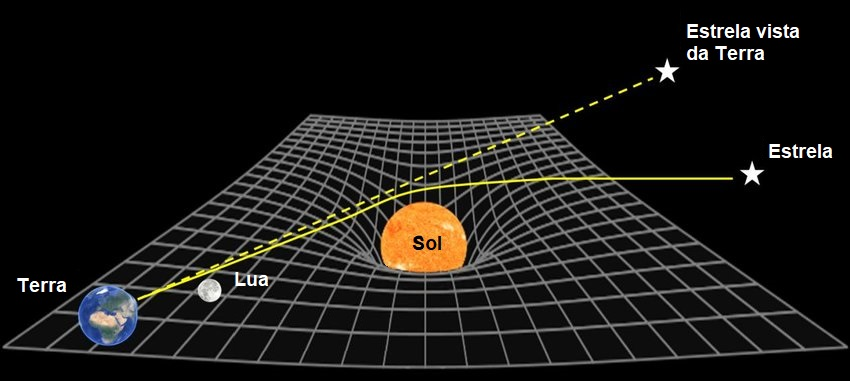
\includegraphics[width=0.85\textwidth]{defle.png}
\end{center}
Fonte: Adaptado de (Paolozzi et al., 2015).
\end{figure}

Tais geodésicas provém da métrica de Schwarzchild $g,$ definida na $4$-variedade $M = \mathbb{R} \times (\mathbb{R}^3 \setminus \overline{B}_{2m}) = \{ (t,r, \theta, \varphi) : r > 2m \}$ dada por
\begin{equation}\label{Sch}
    g = - \left(1 - \dfrac{2m}{r} \right) \dif t^2 + \left(1 + \dfrac{2m}{r} \right)^{-1} \dif r^2 + r (\dif \theta^2 + \mathrm{sen}^2 \theta \dif \varphi^2).
\end{equation}

Esta métrica corresponde ao campo gravitacional externo de um corpo de massa sem carga, não rotativo e esfericamente simétrico (KHURI, 2019). Uma manipulação algébrica fundamentada nos princípios da mecânica lagrangeana nos permite obter a equação da órbita de uma partícula
\[
\left( \frac{\dif r}{\dif \varphi} \right)^{2} = \frac{r^{4}}{b^{2}} - \left( 1 - \frac{2m}{r} \right) \left( \frac{r^{4}}{a^{2}} + r^{2} \right),
\]
cuja solução é 
\begin{equation}\label{Orb}
\varphi = \displaystyle\int \dfrac{1}{\pm r^{2} \sqrt{\dfrac{1}{b^{2}} - \left( 1 - \dfrac{2m}{r} \right) \left( \dfrac{1}{a^{2}} + \dfrac{1}{r^{2}} \right)}}\dif r,
\end{equation}
onde tomamos $a = \frac{h}{c}$ e $b = \frac{cL}{E},$ no qual $h$ é o momento angular específico, $c$ é a velocidade da luz, $L$ é o momento angular e $E$ é a energia total. 

Quando estamos tratando da curvatura da luz, a massa da partícula que estamos considerando vai a $0,$ e a equação da órbita \ref{Orb} se torna
\[
\varphi = \int \frac{\dif r}{r^{2} \sqrt{\dfrac{1}{b^{2}} - \left( 1 - \dfrac{2m}{r} \right) \dfrac{1}{r^{2}}}}
\]
A partir dessa equação, pode-se obter que a deflexão angular aproximada $\delta \varphi$ para a luz é
\[
\delta \varphi \approx \frac{4m}{b} = \frac{4GM}{c^{2}b}
\]

As geodésicas também desempenham um papel importante no estudo dos estados quânticos da luz (TAMATE et al., 2009). Em particular, a partir do uso da esfera de Bloch, que consiste em uma representação geométrica dos estados puros em um sistema quântico de dois níveis, pode-se explorar o comportamento da fase de Pancharatnam da luz por meio do triângulo geodésico, como mostrado na figura \ref{fig:01}.

\begin{figure}[!h]
\begin{center}
\caption{Variação do triângulo geodésico na esfera de Bloch. Aqui, utiliza-se a notação Bra-ket para descrever os estados quânticos.} \label{fig:01}
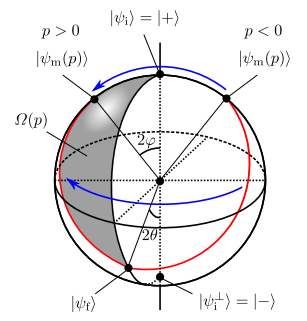
\includegraphics[width=0.5\textwidth]{bloch.png}
\end{center}
Fonte: (Tamate et al., 2009).
\end{figure}

\section{EQUAÇÕES DE CAMPO DA RELATIVIDADE GERAL}

%\textcolor{red}{...a constante cosmológica pode ser omitida ... }
Na Relatividade Geral, as equações de campo são expressões dinâmicas que descrevem a maneira como matéria e energia modificam a geometria do espaço-tempo. Tais equações podem ser deduzidas a partir do princípio variacional, como feito por exemplo em Chandrasekhar (1972). As equações de campo de Einstein que sintetizam a interação da matéria com a geometria do espaço-tempo são dadas por
\[R_{\mu \nu} - \tfrac{1}{2}R g_{\mu \nu} = \frac{8 \pi G }{c^4} T_{\mu \nu},\]
onde $R_{\mu \nu}$ é o tensor de curvatura de Ricci, $R$ é a curvatura escalar, $ g_{\mu \nu}$ é o tensor métrico, $G$ é a constante universal da gravitação de Newton, $c$ é a velocidade da luz no vácuo e $T_{\mu \nu}$ é o tensor energia-momento. Convém salientar que a métrica de Schwarzchild dada em \ref{Sch} é uma solução exata para as equações de campo da Relatividade Geral. 


A formulação variacional permite um melhor entendimento físico da fonte de campo gravitacional e uma maneira mais fácil de englobar outros campos na teoria, ou ainda formular teorias alternativas à Relatividade Geral. De acordo com Will (2014), as equações de campo de Einstein estão em conformidade e possuem um alto grau de aderência com todos os experimentos e observações bem estabelecidos. 

A partir do funcional ação dado por \[\mathcal{S} = \int\limits_{\Omega} \mathcal{L} d^4 x,\] onde $d^4x$ é o elemento de 4-volume, o princípio da mínima ação nos diz que $\delta S = 0,$ de onde pode-se obter as equações de campo. 

Este funcional, no presente caso, pode ser escrito na forma 
\begin{equation}\label{eq:HE}
\mathcal{S} = \int\limits_{\Omega} (\mathcal{L}_G + \kappa\mathcal{L}_M) d^4x,
\end{equation}
onde
\begin{equation}\label{LHE}
\mathcal{L}_G = R \sqrt{-g} \tag{Lagrangiana de Einstein-Hilbert}
\end{equation}
\[
{\delta\mathcal{L}_M \over \delta g^{\mu\nu}} = -\sqrt{-g}T_{\mu\nu}, \tag{Lagrangiana da matéria}
\]
 e $\kappa = 8 \pi G/c^4.$ Podemos reescrever \ref{eq:HE} como
 \[
 S= - {1 \over 2\kappa}\int R \sqrt{-g} d^4x,
 \]
 conhecida como \textit{ação de Hilbert-Einstein}. Fazendo $\delta S = 0$, como já mencionado, obtemos as equações de campo da Relatividade Geral.
 
 Qualquer outra ação que forneça as mesmas equações de movimento será diferente da ação de Einstein-Hilbert por uma derivada total. Por conta disso, a ação de Einstein-Hilbert tem sido a mais utilizada na relatividade geral clássica. (CHAKRABORTY, 2017)
 
Pode-se considerar a representação do espaço de momento da ação de Einstein-Hilbert, a partir da introdução de duas novas variáveis
\[
f^{ab} = \sqrt{-g}g^{ab}; \quad N^a_{bc} = Q^{ad}_{be} \Gamma^{e}_{cd} + Q^{ad}_{ce}\Gamma_{bd}^e = -\Gamma_{bc}^a + \dfrac{1}{2} \left( \Gamma^d_{bd} \delta^a_c + \Gamma^d_{cd} \delta^a_b \right),
\]
onde $f^{ab}$ é o tensor densidade, e $N^a_{bc}$ representa uma combinação linear de conexões. Note que a expressão acima é aplicável para qualquer número de dimensões do espaço-tempo, pois 
\[
Q^{ab}_{cd} = \dfrac{1}{2} \left( \delta^a_c \delta^b_d  - \delta^a_d \delta^b_c \right)\]
independe da dimensão $D$ do espaço-tempo.

O tensor de Ricci pode ser representado em termos de $N^a_{bc}$ por 
\[
R_{ab} = - \left( \delta_c N^a_{bc} + N^c_{ad} N^d_{bc} - \dfrac{1}{D-1} N^c_{ac} N^d_{bd} \right).
\]

Estas variáveis podem ser utilizadas no princípio da mínima ação, e a equação \ref{LHE} que descreve a Lagrangiana de Hilbert-Einstein pode ser descrita por
\[
\mathcal{L}_G = R \sqrt{-g} = f^{ab} R_{ab} = -f^{ab} \left( \delta_c N^a_{bc} + N^c_{ad} N^d_{bc} - \dfrac{1}{D-1} N^c_{ac} N^d_{bd} \right).
\]

Tal formulação culmina na representação do espaço de momento da ação de Einstein-Hilbert, que decorre da constatação de que
\[
N^c_{ab} = \partial (\sqrt{-g}R)/\partial(\partial_c f^{ab}).
\]
\section{CONSIDERAÇÕES FINAIS}

A partir dos estudos realizados, constatou-se a importância do uso de fórmulas relacionadas ao cálculo variacional para resolução de problemas clássicos de física relacionados à teoria da relatividade geral, destacando a utilidade de tais métodos para aplicações de situações clássicas desse campo de estudo, como problema da geodésica, em problemas da relatividade geral, como a deflação da luz e as ações de Hilbert-Einstein.

\begin{thebibliography}{99} 

\bibitem{Castro}
CASTRO, L. M. {\bf O Cálculo Variacional e as Curvas Cicloidais}. Dissertação de Mestrado. Universidade de Brasília, 2014.

\bibitem{CHANDRASEKHAR}
CHANDRASEKHAR, S. {\bf On the derivation of Einstein’s field
equations}, American Journal of Physics,v. 40, n. 2, p. 224–234, 1972.

\bibitem{CHAKRABORTY}
CHAKRABORTY, S. {\bf Boundary terms of the Einstein-Hilbert action
}, Fundamental Theories of Physics, 187, p. 43–59, 2017.

\bibitem{Einstein} 
D'INVERNO, R. {\bf Introducing Einstein's Relativity}. Clarendon Press, 1992.

\bibitem{Khuri}
KHURI, M.; SOKOLOWSKY, B.; WEINSTEIN, G. A. {\bf Penrose-type inequality with angular momentum and charge for axisymmetric initial data.} General Relativity and Gravitation v. 51, n. 118, 2019.

\bibitem{Macedo} 
MACEDO, D. L. {\bf Aplicações do Cálculo Variacional: Braqusitócrona e o Princípio
de Fermat}. 2004.

\bibitem{Odzijewicz} 
ODZIJEWICZ, T.; MALINOWSKA, A. B.; TORRES, D. M. T. {\bf Fractional Variational Calculus with Classical and Combined Caputo Derivatives}. Nonlinear Analysis, v. 75, n.3, p. 1507--1515, 2012.

\bibitem{Paolozzi} 
PAOLOZZI A.; PARIS C.; SINDONI G; and TARTAGLIA, A. {\bf The LARES Mission: An Opportunity to Teach General Relativity - Frame Dragging and Lense-Thirring Effect}. In: Proceedings of the 7th International Conference on Computer Supported Education. p. 343--348, 2015

\bibitem{Riewe} 
RIEWE, F. {\bf Mechanics with fractional derivatives} Physics Review, v. 55, n. 1, p. 3581--3592, 1997.


\bibitem{Tamate}
TAMATE, S.; NAKANISHI, T.; KOBAYASHI, H.; KITANO, M. {\bf Geometrical aspects of weak measurements and quantum erasers}, New Journal of Physics, v. 11, n. 9, 2009.


\bibitem{Tausk}
TAUSK, D. V. {\bf Notas de aula de Cálculo Variacional}, {\it Minicurso IF-Instituto de Fisica 2019}, Universidade de São Paulo, 2019.

\bibitem{Will}
WILL, C. M. {\bf The Confrontation between General Relativity and Experiment}, Living Reviews in Relativity, v. 17, n. 4, 2014.
\end{thebibliography}


\end{document}

